\documentclass[a4paper]{scrartcl}
\usepackage{makecell}
\usepackage{multicol}
\usepackage{graphicx}
\usepackage{anysize}
\usepackage{amsmath}
\usepackage{kpfonts}
\usepackage{tabularx}
\usepackage{hyperref}
\usepackage{listings}
\usepackage{color}

\marginsize{25mm}{25mm}{25mm}{25mm}
%---Code-Editor Config ------------------------%
\definecolor{dkgreen}{rgb}{0,0.6,0}
\definecolor{gray}{rgb}{0.5,0.5,0.5}
\definecolor{mauve}{rgb}{0.58,0,0.82}
\definecolor{backcolour}{rgb}{0.95,0.95,0.92}
\lstset{basicstyle=\ttfamily}
\lstset{literate=%
  {Ö}{{\"O}}1
  {Ä}{{\"A}}1
  {Ü}{{\"U}}1
  {ß}{{\ss}}1
  {ü}{{\"u}}1
  {ä}{{\"a}}1
  {ö}{{\"o}}1
  {é}{{\"AC}}1
  {€}{{\"AC}}1
}
\lstset{
	language=Python,				% the language of the code
	basicstyle=\footnotesize,			% the size of the fonts that are used for the code
	numbers=left,					% where to put the line-numbers
	numberstyle=\tiny\color{gray},		% the style that is used for the line-numbers
	stepnumber=1,					% the step between two line-numbers. If it's 1, each line will be numbered
	numbersep=5pt,				% how far the line-numbers are from the code
	backgroundcolor=\color{white},		% choose the background color. You must add \usepackage{color}
	showspaces=false,				% show spaces adding particular underscores
	showstringspaces=false,			% underline spaces within strings
	showtabs=false,				% show tabs within strings adding particular underscores
	frame=single,					% adds a frame around the code
	rulecolor=\color{black},			% if not set, the frame-color may be changed on line-breaks within not-black text (e.g. commens (green here))
	tabsize=2,						% sets default tabsize to 2 spaces
	captionpos=b,					% sets the caption-position to bottom
	breaklines=true,                			% sets automatic line breaking
  	breakatwhitespace=false,       		% sets if automatic breaks should only happen at whitespace
  	title=\lstname,        % show the filename of files included with \lstinputlisting; % also try caption instead of title
  	keywordstyle=\color{blue},          	% keyword style
  	commentstyle=\color{dkgreen},       	% comment style
  	stringstyle=\color{mauve},         		% string literal style
  	escapeinside={\%*}{*)},            		% if you want to add LaTeX within your code
  	morekeywords={*,...}              		% if you want to add more keywords to the set
}

%Header and Footer -----------------------%
\usepackage[headsepline]{scrlayer-scrpage}
\pagestyle{scrheadings}
\clearpairofpagestyles
%\setlength{\headheight}{40.8pt}
\setlength{\headheight}{56pt}
\ihead{IRTM\\ Wi 20/21\\ Assigment 3} 
\ohead{
    Alberto Saponaro - saponaroalberto97@gmail.com\\
    Walter Väth - walter.vaeth@gmail.com\\
    Chong Shen - st143575@stud.uni-stuttgart.de\\
    Xin Pang - st145113@stud.uni-stuttgart.de
}
\ofoot{\pagemark}

%-----------------------------------------------%
%  BEGIN                                        %
%-----------------------------------------------%
\begin{document}
    
\section*{Task 1}
\subsection*{Subtask 1}
\begin{center}
    $w_{t,d}=(1+\log tf_{t,d})*\log \frac{N}{df_t}$
\end{center}
\begin{itemize}
    \item $w_{pens, d_1} = (1+\log 1) * \log \frac{3}{1} \approx  1,1$
    \item $w_{pens, d_2} = $ not in the doc
    \item $w_{pens, d_3} = $ not in the doc
    \item $w_{write, d_1} = (1+\log 1) * \log \frac{3}{3} = 0$
    \item $w_{write, d_2} = (1+\log 1) * \log \frac{3}{3} = 0$
    \item $w_{write, d_3} = (1+\log 1) * \log \frac{3}{3} = 0$
    \item $w_{on, d_1} = (1+\log 1) * \log \frac{3}{3} = 0$
    \item $w_{on, d_2} = (1+\log 1) * \log \frac{3}{3} = 0$
    \item $w_{on, d_3} = (1+\log 1) * \log \frac{3}{3} = 0$
    \item $w_{paper, d_1} = (1+\log 2) * \log \frac{3}{3} = 0$
    \item $w_{paper, d_2} = $ not in the doc
    \item $w_{paper, d_3} = (1+\log 1) * \log \frac{3}{3} = 0$
    \item $w_{pencils, d_1} = $ not in the doc
    \item $w_{pencils, d_2} = (1+\log 1) * \log \frac{3}{1} \approx 1,1$
    \item $w_{pencils, d_3} = $ not in the doc
    \item $w_{envelope, d_1} = $ not in the doc
    \item $w_{envelope, d_2} = (1+\log 1) * \log \frac{3}{1} \approx 1,1$
    \item $w_{envelope, d_3} = $ not in the doc
    \item $w_{ballpens, d_1} = $ not in the doc
    \item $w_{ballpens, d_2} = $ not in the doc
    \item $w_{ballpens, d_3} = (1+\log 1) * \log \frac{3}{1} \approx 1,1$
\end{itemize}

\begin{tabular}{|l|c|c|c|}
    \hline
    \textbf{Terms} & \textbf{$d_1$} & \textbf{$d_2$} & \textbf{$d_3$} \\ \hline
    pens           & 1.1               & 0.0               & 0.0               \\ \hline
    write          & 0.0               & 0.0               & 0.0               \\ \hline
    on             & 0.0               & 0.0               & 0.0               \\ \hline
    paper          & 0.0               & 0.0               & 0.0               \\ \hline
    pencils        & 0.0               & 1.1               & 0.0               \\ \hline
    envelope       & 0.0               & 1.1               & 0.0               \\ \hline
    ballpens       & 0.0               & 0.0               & 1.1               \\ \hline
\end{tabular}
\newline
$\overrightarrow{d_1} = (1.1, 0.0, 0.0, 0.0, 0.0, 0.0, 0.0)$\\
$\overrightarrow{d_2} = (0.0, 0.0, 0.0, 0.0, 1.1, 1.1, 0.0)$\\
$\overrightarrow{d_3} = (0.0, 0.0, 0.0, 0.0, 0.0, 0.0, 1.1)$\\

\subsection*{Subtask 2}
$w_{ballpens, q} = (1+\log 1) * \log \frac{3}{1} \approx 1,1$\\
$w_{envelope, q} = (1+\log 1) * \log \frac{3}{1} \approx 1,1$\\

$\overrightarrow{q}=(0.0, 0.0, 0.0, 0.0, 0.0, 1.1, 1.1)$\\

$SIM(\overrightarrow{q}, \overrightarrow{d_1}) = \frac{\overrightarrow{q}*\overrightarrow{d_1}}{|\overrightarrow{q}|*|\overrightarrow{d_1}|}
= 0$\\
$SIM(\overrightarrow{q}, \overrightarrow{d_2}) = \frac{\overrightarrow{q}*\overrightarrow{d_2}}{|\overrightarrow{q}|*|\overrightarrow{d_2}|}
= \frac{1.21}{49} \approx  0.025$\\
$SIM(\overrightarrow{q}, \overrightarrow{d_3}) = \frac{\overrightarrow{q}*\overrightarrow{d_3}}{|\overrightarrow{q}|*|\overrightarrow{d_3}|}
= \frac{1.21}{49} \approx 0.025$\\

\begin{tabular}{|c|c|r|}
    \hline
    \textbf{Rank} & \textbf{Doc} & \multicolumn{1}{c|}{\textbf{SIM}} \\ \hline
    1             & 2            & 0.025                                   \\ \hline
    1             & 3            & 0.025                             \\ \hline
    2             & 1            & 0                         \\ \hline
\end{tabular}


\pagebreak
\section*{Task 3}

\begin{itemize}
    \item $Precision = \frac{TPs}{TPs+FPs}$
    \item $Recall = \frac{TPs}{TPs+FNs}$
\end{itemize}

\begin{center}
    \begin{tabular}{@{}llll@{}}
    \hline
    \textbf{k} & \textbf{Result Set}           & \textbf{Precision} & \textbf{Recall} \\ \hline
    1          & 127                           & 1.0                & 0.2             \\
    2          & 127, 9                        & 0.5                & 0.2             \\
    3          & 127, 9, 10                    & 0.33               & 0.2             \\
    4          & 127, 9, 10, 2                 & 0.5                & 0.4             \\
    5          & 127, 9, 10, 2, 35             & 0.4                & 0.4             \\
    6          & 127, 9, 10, 2, 35, 32         & 0.33               & 0.4             \\
    7          & 127, 9, 10, 2, 35, 32, 41     & 0.43               & 0.6             \\
    8          & 127, 9, 10, 2, 35, 32, 41, 64 & 0.5                & 0.8             \\ \hline
    \end{tabular}
    
    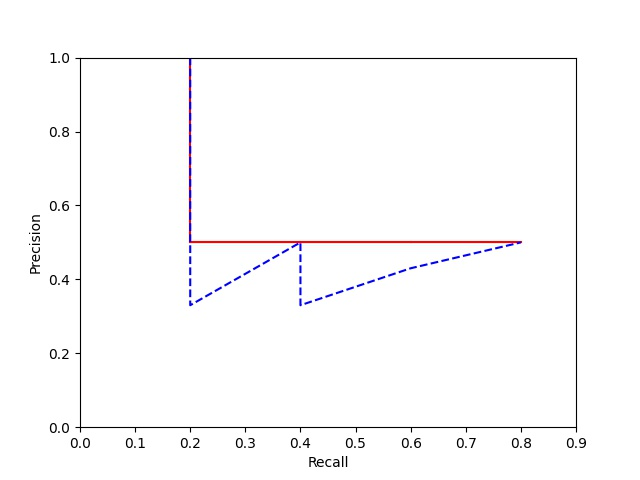
\includegraphics[width=.7\textwidth]{img/fig.jpg}
\end{center}

\section*{Task 4}

An advantage of using IDF over stop word list is that
you don't have a fixed set of words that maybe must be expanded in the future.
Expanding a stop word list will change all the weights as a consequence.
Due to the Zipf's law if a term is contained in all the documents is most likely to be a stop word.
If the IDF value of a term is 0(occurs in all documents) than will have the same effects as if it was included in the stop word lists.
\\
Advantage of using stops words lists are that we could prevent the calculation of the IDF for stops
and we can be more precise not including words that maybe occurs in every document but aren't stops.

\section*{Programming Task}

\subsection*{Subtask 1}

The ranking method implemented is based on tf-matching-score with log frequency weighting.
Given a query the method \textbf{tf\_matching\_scores} will output a dictionary with the tf-matching-score for all relevant documents.
A \textit{relevant} document contains at least one term of the query at least one time.\\

In the implementation we iterate through the documents to calculate the log frequency weights for each term in the document ($W_{t,d}$) 
and then we calculate the tf-matching-score for each document. We use a log tf because the relevance does not increase proportionally with term frequency.
After that we rank the results with the method \textbf{ranking\_table} which ranks the results and print a ranking table to the terminal.




\subsubsection*{Code}
\begin{lstlisting}[language=python]
    #...
    
    def tf_matching_scores(self, query: str) ->dict:
    """Calculate tf-matching-score for all documents given the query.

    Args:
        query (str): Query against which we calculate the document's score

    Returns:
        dict: For each document the tf-matching-score 
    """
    query = query.lower()
    query = query.split()
    
    docs_weights = {}
    tf_matching_scores = {}
    
    # retrive the news title and text to calculate tf-weights
    with open( self.filename, 'r' ) as file:
        reader = csv.reader(file, delimiter = '\t')
        
        #iterate through each row of the table
        for row in reader:
            # skip table header
            if( row[0] == 'id' ): continue
            
            #(doc_id, url, pub_date, title, news_text) = row
            doc_ID = int(row[0])
            news_title = row[-2]
            news_text = row[-1]

            docs_weights.update({doc_ID: []})

            tokenizer = nltk.RegexpTokenizer(r"\w+")
            normalized_news_title = tokenizer.tokenize(news_title.lower())
            normalized_news_text = tokenizer.tokenize(news_text.lower())

            news_terms = normalized_news_title + normalized_news_text
            
            for term in query:
                
                if( term in news_terms ):
                    log_tf = math.log(dict(Counter(news_terms))[term])
                    docs_weights[doc_ID].append(1 + log_tf)
                else: 
                    docs_weights[doc_ID].append(0)
            
            # delete all documents that are not relevant to the query
            if( docs_weights[doc_ID] == [0,0] ):
                docs_weights.pop(doc_ID)

            #calculate tf-matching-scores
            for doc_ID in docs_weights:
                tf_matching_scores.update( {doc_ID: sum(docs_weights[doc_ID])} )
    
    return tf_matching_scores

def ranking_table(self, scores: dict):
    """Print a ranking table given a dictionary of scores

    Args:
        scores (dict): Datastructure that contains all scores
    """
    sorted_dict = sorted(scores.items(), key=itemgetter(1), reverse=True)
    ranked_list = []
    rank = 0
    old_score = 0
    
    for items in sorted_dict:
        doc_ID = items[0]
        score = items[-1]

        # don't rank if the score is zero
        if( score == 0 ): continue
        
        if( old_score == score):
            ranked_list.append((rank, doc_ID, score))
        else:
            rank += 1
            ranked_list.append((rank, doc_ID, score))
            old_score = score
    
    # print ranking table
    #print only top 10
    print("Rank \t", "Doc \t", "Score")
    print("-"*30)
    counter = 0
    for row in ranked_list:
        if ( counter > 9 ): break
        rank, doc_ID, score = row
        print(rank, "\t", doc_ID, "\t", round(score, 5))
        counter += 1
    


if __name__ == "__main__":
filename = 'assignment3/code/postillon.csv'
search = Search(filename=filename)

print("\n"*3)
print("1. Query: olympische sportbund")
scores = search.tf_matching_scores("olympische sportbund")
search.ranking_table(scores)

print("\n"*3)
print("2. Query: rot wein")
scores = search.tf_matching_scores("rot wein")
search.ranking_table(scores)

print("\n"*3)
print("3. Query: kinder sind faul")
scores = search.tf_matching_scores("kinder sind faul")
search.ranking_table(scores)

\end{lstlisting}

\subsubsection*{OUTPUT:}
\begin{lstlisting}
    1. Query: olympische sportbund
Rank     Doc     Score
------------------------------
1        4194    2.69315
2        276     2.60944
3        1632    2.09861
4        3925    2.0
4        4759    2.0
5        2018    1.69315
5        2146    1.69315
5        4990    1.69315
6        228     1.0
6        548     1.0




2. Query: rot wein
Rank     Doc     Score
------------------------------
1        165     2.38629
2        1063    1.69315
2        1210    1.69315
2        1872    1.69315
2        2212    1.69315
2        2332    1.69315
2        2837    1.69315
2        2978    1.69315
2        3712    1.69315
3        150     1.0




3. Query: kinder sind faul
Rank     Doc     Score
------------------------------
1        3763    5.4012
2        2789    5.07944
3        1827    4.89037
4        583     4.77259
5        4228    4.60944
6        1494    4.19722
6        2658    4.19722
7        2011    4.07944
8        150     3.94591
8        4887    3.94591
\end{lstlisting}


\end{document}